%极限

\begin{frame}
	\frametitle{第三讲、数列的极限}
	\linespread{1.5}
	\begin{enumerate}
	  \item {\bf 内容与要求}{\color{blue}( \S2.1-2.2 )}
	  \begin{itemize}
	    \item 理解数列的概念
	    \item 掌握数列极限的“$\e-N$”定义
	    \item 熟练掌握数列极限的基本性质
	  \vspace{1em}
	  \end{itemize}
	  \item {\bf 课后练习:}
	  \begin{itemize}
	    \item 书面作业:{\b 习题2.1:2,6(2,3),7,8}
	    \item 思考题:{\b 习题2.1:11,12,15}
	  \end{itemize}
	\end{enumerate}
\end{frame}

\begin{frame}{数列}
	\linespread{1.2}\pause
	\begin{itemize}
	  \item $1,2,3,4,\ldots,n,\ldots$\pause 
	  \item $1,3,5,7,\ldots,2n-1,\ldots$\pause 
	  \item $1,\df 12,\df 13,\df 14,\ldots,\frac 1n,\ldots$\pause 
	  \item $1,-1,1,-1,\ldots,(-1)^n,\ldots$\pause 
	\end{itemize} 
	\begin{block}{数列的定义}
		$$f:\mathbb{N}\to\mathbb{R}$$
	\end{block}\pause 
	{\bf 问题:}数列与集合有哪些不同?
\end{frame}

\begin{frame}{数列的极限}
	\linespread{1.2}\pause 
	{\bf 极限:}\pause 一种无限靠近的趋势\pause 
	\begin{enumerate}
	  \item 对于数列而言,无限靠近的趋势意味着什么?\pause 
	  \item 如何从数学上严格表达这种趋势?\pause 
	\end{enumerate}
	\begin{block}{{\bf 定义2.1.2}\hfill P48}\pause 
		称数列$\{a_n\}$以$a$为极限\pause 
% 		(或$\{a_n\}$\alert{收敛}于$a$)
		,是指:\pause {\bb
		$\forall\e>0$,\pause $\exists N>0$,\pause 对$\forall n>N$,\pause 有
		$|a_n-a|<\e$}。\pause 记为 $$\lim_{n\to\infty}a_n=a\quad\mbox\pause
		{\mbox{或}}\quad a_n\to a\;(n\to\infty)$$
	\end{block}
\end{frame}

% \begin{frame}[empty]
% 	\linespread{1.2}
% 	\begin{block}{定义}
% 		{\bb $\forall\e>0$,$\exists N>0$,使对$\forall n>N$,有
% 		$|a_n-a|<\e$}
% 	\end{block}\pause 
% 	\begin{itemize}
% 	  \item {\ba {“$a$确定”}}\pause ($a\ne\pm\infty$)\pause 
% 	  \item {\ba {“$\e$要小”}}\pause 
% 	  \begin{itemize}
% 	    \item “$\forall\e$”\pause $\Leftrightarrow$“对任意小的$\e$”\pause 
% 	  \end{itemize}
% 	  \item {\ba {“$N$要大”}}\pause 
% 	  \begin{itemize}
% 	    \item $N$由$\e$决定\pause 	    
% 	    \item “存在$N$”$\pause \Leftrightarrow$“存在充分大的$N$”\pause 
% 	  \end{itemize}
% 	  \item {\ba{不等式可放缩}}
% 	  \begin{itemize}
% 	    \item “$|\ldots|<\e$”\pause $\Leftrightarrow$“$|\ldots|<C\e$”,$C$为常数\pause 
% 	  \end{itemize}
% 	  \item {\ba{次序不能变!}}
% 	\end{itemize}
% % 	\hline
% % 	\begin{center}
% % 	{\ba{“随着$n$越来越大,$a_n$与$a$的差将越来越小”}}
% % 	\end{center}
% % 	例如:$a_n=(-1)^n/n$
% \end{frame}

\begin{frame}{等价说法}
	\linespread{1.2}
	\begin{center}
		\alert{$\forall\e>0$,$\exists N>0$,对$\forall n>N$,有
		$|a_n-a|<\e$}
	\end{center}\pause 
	以下与该定义等价的说法是:\pause  
	\begin{enumerate}
	  \item $\forall\e>0$,$\exists N\in\mathbb{N}$,对$\forall
	  n>N$,$|a_n-a|<\e$\pause \hfill\alert{$\surd$}\pause 
	  \item $\forall\e>0$,$\exists N>0$,对$\forall
	  n>N$,$|a_n-a|\leq\e$\pause \hfill\alert{$\surd$}\pause 
	  \item $\exists N>0$,对$\forall\e>0$,$\forall
	  n>N$,$|a_n-a|<\e$\pause \hfill\alert{$\times$}\pause 
	  \item $\forall\e>0$,仅有有限多个$n$,使得$|a_n-a|\geq\e$\pause
	  \hfill\alert{$\surd$}\pause 
	  \item $\forall\e>0$,定有无穷多个$n$,使得$|a_n-a|<\e$\pause
	  \hfill\alert{$\times$}\pause 
	  \item $\forall\e>0$,要使$|a_n-a|<\e$,只须$n$充分大\pause \hfill\alert{$\surd$}
	\end{enumerate}
\end{frame}

% \begin{frame}{等价定义}
% 	\linespread{1.2}
% 	\begin{center}
% 		\alert{$\forall\e>0$,$\exists N>0$,对$\forall n>N$,有
% 		$|a_n-a|<\e$}
% 	\end{center}
% 	以下与该定义等价的说法是: 
% 	\begin{enumerate}
% 	  \item {\b $\forall\e>0$,$\exists N\in\mathbb{N}$,对$\forall
% 	  n>N$,$|a_n-a|<\e$}
% 	  \item {\b $\forall\e>0$,$\exists N>0$,对$\forall
% 	  n>N$,$|a_n-a|\leq\e$}
% 	  \item \alert{\sout{$\exists N>0$,对$\forall\e>0$,$\forall
% 	  n>N$,$|a_n-a|<\e$}}
% 	  \item {\b $\forall\e>0$,仅有有限多个$n$,使得$|a_n-a|\geq\e$}
% 	  \item \alert{\sout{$\forall\e>0$,定有无穷多个$n$,使得$|a_n-a|<\e$}}
% 	  \item {\b $\forall\e>0$,要使$|a_n-a|<\e$,只须$n$充分大}
% 	\end{enumerate}
% \end{frame}

\begin{frame}
	\linespread{1.2}
	\begin{block}{定义}
		{\bb $\forall\e>0$,$\exists N>0$,对$\forall n>N$,有
		$|a_n-a|<\e$}
	\end{block}\pause 
	\begin{itemize}
	  \item $a\in\mathbb{R}$是一个确定的数\pause (\alert {不能是$\pm\infty$})\pause 
	  \item “$\forall\e>0$”应该理解为\alert{“对任意小的$\e>0$”},\pause
	  表示$a_n$可以无限接近$a$\pause
	  \item $N$是由$\e$决定的数,\pause “存在$N>0$”\pause
	  应该理解为\alert{“存在充分大的$N(\e)$}”;\pause 
	   如果$N$能够满足定义,\pause 任意比$N$大的数都能够满足定义;\pause 通常$\e$取得越小,
	  $N$需要取得越大\pause 
	  \item “$|a_n-a|<\e$”\pause 可替换为\alert{“$|a_n-a|<C\e$”},\pause 其中$C>0$是为常数
	\end{itemize}
% 	\hline
% 	\begin{center}
% 	{\ba{“随着$n$越来越大,$a_n$与$a$的差将越来越小”}}
% 	\end{center}
% 	例如:$a_n=(-1)^n/n$
\end{frame}

\begin{frame}
	\linespread{1.5}
	\begin{block}{{\bf 补充定理}}
		$\limn a_n=a$等价于:给定$C>0$,对$\forall\e>0$,$\exists N>0$,对
		$\forall n>N$,有
		$$|a_n-a|<C\e$$
	\end{block}
\end{frame}

\begin{frame}
	\linespread{1.4}
	\begin{block}{定义}
		{\bb $\forall\e>0$,$\exists N>0$,使对$\forall n>N$,有
		$|a_n-a|<\e$}
	\end{block}\pause
	\begin{exampleblock}{{\bf 例1:}证明}
		$$\lim\limits_{n\to\infty}(-1)^n\displaystyle\frac{1}{\,n^2\,}=0$$\pause
% 		\hline
	\end{exampleblock}
	\pause
	\begin{exampleblock}{{\bf 课堂练习:}证明}
		$$\limn\df{n}{n+1}=1$$
	\end{exampleblock}
% 		{\bf 证:}
% 		对{\ba{
% 		$\forall\e>0$}},\pause{\alert{取$N=\displaysytle\frac{1}{\,\e\,}$}},\pause
% 		 则{\alert{对$\forall n>N$}},\pause 总有
% 		$${\alert{
% 		\left|(-1)^n\frac{1}{\,n^2\,}-0\right|}}\pause
% 		=\frac{1}{\,n^2\,}\pause \le\frac{1}{\,n\,}\pause {\ba{
% 		<}}\frac{1}{\,N\,}\pause ={\ba {\e}},$$ \pause 即证。
\end{frame}

\begin{frame}
	\linespread{1.5}
% % 	\begin{exampleblock}{{\bf 例2:}证明\hfill P55-习题6(4)}
% 		$$\limn\df{n^2-n+2}{3n^2+2n-4}=\df 13$$
% 	\end{exampleblock}\pause 
	\begin{exampleblock}{{\bf 例2:}证明\hfill P54-习题4}
		若$\limn a_n=a$,则$\limn|a_n|=a$。
	\end{exampleblock}
	\bigskip\pause 
	\begin{exampleblock}{{\bf 例3:}证明}
		若$|q|<1$为常数,则数列$\{q^n\}$极限存在。
	\end{exampleblock}
	\pause
	\alert{\bf 思考:}若$|q|>1$,如何证明$\{q^n\}$极限不存在?
\end{frame}

\begin{frame}{反面说法}
	\linespread{1.5}\pause 
	\begin{block}{{\bf 正面:}$\{a_n\}$以$a$为极限}
		{ $\forall\e>0$,$\exists N>0$,使对$\forall n>N$,有
		$|a_n-a|<\e$}
	\end{block}\pause 
	\begin{alertblock}{{\bf 反面:}$\{a_n\}$不以$a$为极限}\pause 
		{\b $\exists\e_0>0$,\pause 对$\forall N>0$,\pause $\exists
		n_0>N$,\pause 使得$|a_{n_0}-a|\geq\e_0$ }
	\end{alertblock}\pause 
	\begin{exampleblock}{{\bf 例4}\hfill P50-例5}
		证明:数列$\{(-1)^n\}$无极限。
	\end{exampleblock}
\end{frame}

\begin{frame}{数列极限的基本性质}
	\linespread{1.5}
	\begin{enumerate}\pause 
	  \item {\bf 唯一性}\pause 
	  \item {\bf 有界性}\pause 
	  \item {\bf 保号性}\pause 
	  \item {\bf 极限的四则运算}
	\end{enumerate}
\end{frame}

\begin{frame}{唯一性}
	\linespread{1.2}\pause 
	\begin{block}{{\bf 定理2.1.1}\hfill P52}
		数列$\{a_n\}$若存在极限,则极限必唯一。
	\end{block}\pause 
	\begin{center}
		\resizebox{!}{4.8cm}{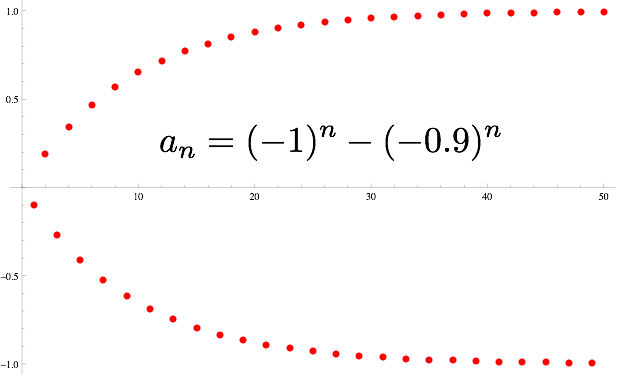
\includegraphics{./images/ch2/1-0.9n.jpg}}
	\end{center}
\end{frame}

\begin{frame}{有界性}
	\linespread{1.2}\pause 
	\begin{block}{{\bf 定理2.1.2}\hfill P52}
		数列$\{a_n\}$若存在极限,则$\{a_n|n\in\mathbb{Z}\}$必有界。
	\end{block}\pause 
	\begin{center}
		\resizebox{!}{4.8cm}{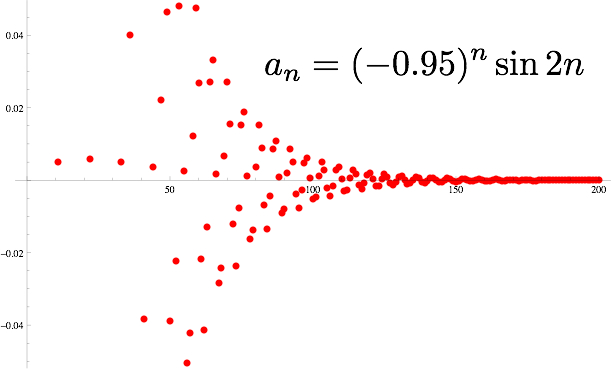
\includegraphics{./images/ch2/sin2nn.jpg}}
	\end{center}
\end{frame}

\begin{frame}{保号性}
	\linespread{1.4}\pause 
	\begin{block}{{\bf 定理2.1.3}\hfill P53}\pause 
		设$\lim\limits_{n\to\infty}a_n>0$,\pause 则$\exists N>0$,\pause
		对$\forall n>N$,$a_n>0$ \end{block}\pause 
	\begin{block}{{\bf 推论}\hfill P54}\pause 
		\begin{enumerate}
		  \item 设对$\forall n\in\mathbb{N}$,$a_n\geq
		  0$,\pause $\lim\limits_{n\to\infty}a_n=a$,\pause 则$a\geq 0$\pause 
		  \item 设$\lim\limits_{n\to\infty}a_n=a\ne
		  0$,\pause 则$\exists N$,当$n>N$时,$|a_n|>|a|/2$\pause 
		  \item
		  设$\lim\limits_{n\to\infty}a_n=a$,\pause 且最多有有限个$a_n$小于零,\pause 则$a\geq 0$
		\end{enumerate}	
	\end{block}
\end{frame}

\begin{frame}{极限的四则运算}
	\linespread{1.4}\pause 
	\begin{block}{{\bf 定理2.2.1}\hfill P57}\pause 
		设数列$\{a_n\},\{b_n\}$分别以$a,b\,(b\ne 0)$为极限,\pause 则
		\begin{enumerate}
		  \item $\lim\limits_{n\to\infty}(a_n\pm b_n)=a\pm b$\pause 
		  \item $\lim\limits_{n\to\infty}a_nb_n=ab$\pause 
		  \item
		  $\lim\limits_{n\to\infty}\displaystyle\frac{a_n}{b_n}=\displaystyle\frac{a}{\,b\,}$
		\end{enumerate}
	\end{block}\pause 
	\begin{exampleblock}{{\bf 例5:}计算极限\hfill P58-例2}
		$$\limn\df{2n^6+3n^4-n+10}{n^6+n^4+1}$$
	\end{exampleblock}
\end{frame}

\begin{frame}
	\linespread{2}\pause 
	\begin{exampleblock}{{\bf 例6}\hfill P58-例1}
		设$\limn(a_n+b_n)=1$,$\limn(a_n-b_n)=3$,证明$\{a_n\},\{b_n\}$收敛,并求其值。
	\end{exampleblock}
	\bigskip\pause 
	\begin{exampleblock}{{\bf 例7}\hfill P59-例3}
		设$q$为常数,且$|q|>1$,证明$\limn q^n$不存在
	\end{exampleblock}
\end{frame}

\begin{frame}[<+->]{小结}
	\linespread{1.5}
	\begin{enumerate}
	  \item {\bf 定义:$\limn a_n=a$}
	  \begin{itemize}
	    \item $\forall\e>0$,$\exists N>0$,使对$\forall n>N$,有
		$|a_n-a|<\e$
		\item 反面说法
	  \end{itemize}
	  \item {\bf 基本性质}
	  \begin{itemize}
	    \item 唯一性、有界性、保号性
	    \item 利用四则运算简化极限计算
	  \end{itemize}
	\end{enumerate}
	\pause
% 	\vspace{1em}
	\pause
	\begin{exampleblock}{课后习题}
	  \begin{itemize}
	    \item 书面作业:{\b 习题2.1:2,6(2,3),7,8}
	    \item 思考题:{\b 习题2.1:11,12,15}
	  \end{itemize}
	\end{exampleblock}
\end{frame}

\begin{frame}{课堂练习}
	\linespread{1.5}
\end{frame}

\begin{frame}{课堂练习}
	\linespread{1.5}
	\begin{exampleblock}{{\bf 例8:}计算极限\hfill }
		$$\limn\df{\cos^n\theta-\sin^n\theta}{\cos^n\theta+\sin^n\theta}\quad
	  	(0\leq\theta\leq\df{\pi}{2})$$
	\end{exampleblock}
	\bigskip
	\pause
% 	\begin{exampleblock}{{\bf 例9}\hfill }
% 		$f(x)=\limn\df{x^{2n}+x^n+x}{x^{2n}+1}$,求$f(x)$的表达式。
% 	\end{exampleblock}
	\begin{exampleblock}{{\bf 例9}\hfill }
		设$a_n>0(n\in\mathbb{N})$,$\limn a_n=a$,证明:
		$$\limn\sqrt{a_n}=\sqrt a$$
	\end{exampleblock}
\end{frame}

% \begin{frame}{title}
% 	\linespread{1.2}
% 	\begin{block}{sample}
% 		this is
% 	\end{block}
% \end{frame}